\documentclass[../Main.tex]{subfiles}

\begin{document}
In this chapter, we will solve the TISE in 3 cases:
\begin{enumerate}
    \item Bound states, where the particle cannot escape to infinity.
    \item The free particle, with no potential $U(x)$
    \item Scattering states
\end{enumerate}
\section{Bound States}
\subsection{Infinite Potential Well}
Consider a potential of the form:
\begin{equation*}
    U(x) =
    \begin{cases}
        0 & |x| \leq a \\
        \infty & |x| > a
    \end{cases}
\end{equation*}
Then for $|x| > a$, we must have that $\chi(x) = 0$. Therefore, consider $|x| \leq a$. Consider the TISE:
\begin{equation*}
    \chi''(x) + \frac{2mE}{\hbar^2} \chi(x) = 0
\end{equation*}
Then since $E \geq 0$, we set $\frac{2mE}{\hbar^2} = k^2$ to get solutions:
\begin{equation*}
    \chi(x) = A\sin(kx) + B\cos(kx)
\end{equation*}
We need to impose the boundary condition $\chi(\pm a) = 0$. This gives that $A\sin(ka) = 0$ and $B\cos(ka) = 0$. There are two options:
\begin{itemize}
    \item $A = 0, \cos(ka) = 0$, this gives a set of values, $k = k_n = \frac{n\pi}{2a}$ for odd $n$.
    \item $B = 0, \sin(ka) = 0$ and here we have $k_n = \frac{n\pi}{2a}$ for even $n$.
\end{itemize}
The energy eigenvalues are $E_n = \frac{\hbar^2 k_n^2}{2m} = \frac{\hbar^2 \pi^2}{8ma^2}n^2$. To determine $A$ and $B$, we require normalisation of the $\chi_n$. For this, we find $A = B = a^{-\frac12}$.

The full solution is:
\begin{equation*}
    \chi_n(x) =
    \begin{cases}
        a^{-\frac12} \sin(\frac{n\pi x}{2a}) & n \text{ even} \\
        a^{-\frac12} \cos(\frac{n\pi x}{2a}) & n \text{ odd}
    \end{cases}
\end{equation*}
\begin{remarks}
    \item The ground state has a non-zero energy. This is contrary to classical mechanics.
    \item As $n \to \infty$, we find that the particle can be anywhere, which corresponds to the classical interpretation, where the probability a particle is at $x$ is inversely proportional to the particle's velocity at $x$.
    \item We only require $\chi(x)$ to be twice differentiable if $U(x)$ is finite. In this case, we did not require $\chi(x)$ to be twice differentiable because the potential $U(x)$ was infinite.
\end{remarks}
\begin{proposition}
    If a quantum system has non-degenerate eigenstates then if $U(x) = U(-x)$, the eigenfunctions of $\hat{H}$ must be either odd or even functions.
    \label{propOddEvenStates}
\end{proposition}
\begin{proof}
    If $U(x) = U(-x)$ then the TISE is invariant under $x \mapsto -x$. Therefore, if $\chi(x)$ is a solution with eigenvalue $E$, $\chi(-x)$ must also be a solution with eigenvalue $E$. Since the system has non-degenerate eigenstates, $\chi(x)$ must be equivalent to $\chi(-x)$:
    \begin{equation*}
        \chi(x) = \lambda\chi(-x),~|\lambda| = 1
    \end{equation*}
    But by rotating $\chi(x)$ and $\chi(-x)$ to be real, we have that $\lambda = \pm 1$, so:
    \begin{equation*}
        \chi(x) = \pm\chi(-x)
    \end{equation*}
    That is, $\chi$ is either odd or even.
\end{proof}
\subsection{Finite Potential Well}
Consider instead a \underline{finite potential well},
\begin{equation*}
    U(x) =
    \begin{cases}
        0 & |x| \leq a \\
        U_0 & |x| > a
    \end{cases}
\end{equation*}
We will only look at bound states, with $E < U_0$. If not, the particle could escape out of the well which will be discussed later.

By proposition~\ref{propOddEvenStates}, we have that $\chi$ must be odd or even. We will consider only even states, because odd states are found on the second example sheet. Let $\chi(x) = \chi(-x)$, and consider:
\begin{equation*}
    \begin{cases}
        -\frac{\hbar^2}{2m}\chi''(x) = E\chi(x) & |x| \leq a \\
        -\frac{\hbar^2}{2m}\chi''(x) = (E - U_0)\chi(x) & |x| > a
    \end{cases}
\end{equation*}
Now solving inside the well gives the solution:
\begin{equation*}
    \chi(x) = A\sin(kx) + B\cos(kx),~k = \sqrt{\frac{2mE}{\hbar^2}}
\end{equation*}
Then for an even solution we get $A = 0$, so $\chi(x) = B\cos(kx)$.

Solving outside the well gives the solution:
\begin{equation*}
    \chi(x) = Ce^{\bar{k}x} + De^{-\bar{k}x},~\bar{k} = \sqrt{\frac{2m(U_0 - E)}{\hbar^2}} 
\end{equation*}
Then we require that $\chi$ can be normalised. For $\chi(\infty) \to 0$, require $C = 0$ when $x > a$. Similarly require $D = 0$ when $x < -a$. Our function is now:
\begin{equation*}
    \chi(x) =
    \begin{cases}
        Ce^{\bar{k}x} & x < -a \\
        B\cos(kx) & |x| \leq a \\
        De^{-\bar{k}x} & x > a
    \end{cases}
\end{equation*}
Now we impose continuity of $\chi$ and its derivative at $x = \pm a$. Note that $\chi$ is even so $C = D$.
\begin{align}
    Ce^{-\bar{k}a} &= B\cos(ka) \label{eqnFPWellEqns} \\
    -\bar{k} C e^{-\bar{k}a} &= -kB\sin(ka) \nonumber
\end{align}
Then taking the ratio of these equations gives $k\tan(ka) = \bar{k}$. We also require that $k^2 + \bar{k}^2 = \frac{2mU_0}{\hbar^2}$. Rescaling using $\xi = ka, \eta = \bar{k} a$,
\begin{align*}
    \xi \tan(\xi) &= \eta
    \xi^2 + \eta^2 = r_0^2
\end{align*}
Here $r_0 = \frac{2mU_0a^2}{\hbar^2}$.
\begin{figure}
    \centering
    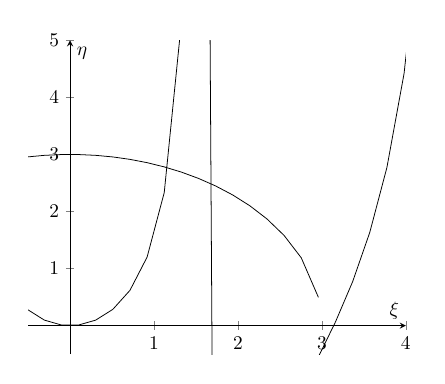
\begin{tikzpicture}[scale=0.7]
        \begin{axis}[
            axis lines=middle,
            xmin=-0.5,xmax=4,ymin=-0.5,ymax=5,
            trig format=rad,
            xlabel={$\xi$},
            ylabel={$\eta$}
        ]
            \addplot[samples=50] {x * tan(x)};
            \addplot[samples=50] {(9 - x^2)^(1/2)};
        \end{axis}
    \end{tikzpicture}
    \caption{Solution of Finite Potential Well}
    \label{figFPWellSoln}
\end{figure}
Then the eigenvalues of $\bar{H}$ correspond to the points of intersection in figure~\ref{figFPWellSoln}.

\begin{remarks}
    \item We can verify that as $U_0 \to \infty$, we get the solutions for the infinite potential well.
    \item There is a second unused condition in equation~\ref{eqnFPWellEqns}. This is used to find $C$ in terms of $B$.
    \item We can determine $B$ by normalising.
\end{remarks}
\subsection{Quantum Harmonic Oscillator}
Consider a potential:
\begin{equation*}
    U(x) = \frac12 k x^2
\end{equation*}
Here $k \in \R, k > 0$ is the elastic constant of the system.
In classical mechanics, we would find the solution:
\begin{equation*}
    x(t) = A\sin(\omega t) + B\cos(\omega t),~\omega = \sqrt{\frac{k}{m}}
\end{equation*}
In Quantum Mechanics, we have the TISE:
\begin{equation}
    \frac{-\hbar^2}{2m}\chi'' + \frac{1}{2}m\omega^2 x^2 \chi = E\chi
    \label{eqnQHMTISE}
\end{equation}
Then consider the change of variables $\xi^2 = \frac{m\omega}{\hbar}\chi^2, \epsilon = \frac{2E}{\hbar \omega}$. Substituting this into equation~\ref{eqnQHMTISE}:
\begin{equation}
    -\frac{d^{2}\chi(\xi)}{d\xi^{2}} + \xi^2 \chi(\xi) = \epsilon\chi(\xi)
    \label{eqnQHMScaledTISE}
\end{equation}
Now we can solve this by starting from a particular solution with $\epsilon = 1$,
\begin{equation}
    \chi_0(\xi) = e^{-\frac{\xi^2}{2}}
    \label{eqnQHMPartSoln}
\end{equation}
Then we can use a trial form $\chi_n(\xi) = f(\xi) e^{-\frac{\xi^2}{2}}$. This gives the differential equation:
\begin{equation}
    -\frac{d^{2}f}{d\xi^{2}} + 2\xi \frac{df}{d\xi} + (1 - \epsilon)f = 0
    \label{eqnQHMTrialEquation}
\end{equation}
The best way to solve this is with a power series,
\begin{equation}
    f(\xi) = \sum_{n=0}^{\infty} a_n \xi^n
    \label{eqnQHMSeries}
\end{equation}
Substituting this in gives:
\begin{align*}
    0 &= -\sum_{n=0}^{\infty} n(n-1) \xi^{n-2} + 2\sum_{n=0}^{\infty} na_n \xi^n + (1 - \epsilon) \sum_{n=0}^{\infty} a_n \xi^n \\
    &= \sum_{n = 0}^{\infty} \left[(n+1)(n+2) a_{n+2} - 2n a_n + (\epsilon - 1) a_n\right]
\end{align*}
Then since each term must be 0 individually,
\begin{equation}
    a_{n+2} = \frac{2n - \epsilon + 1}{(n+1)(n+2)}
    \label{eqnQHMRecurRelation}
\end{equation}
We know that, for a symmetric potential, the function must either be odd or even. Therefore, either $a_{2n+1} = 0$, to give $f(\xi) = f(-\xi)$; or, $a_{2n} = 0$ to give $f(\xi) = -f(-\xi)$.
\begin{proposition}
    If, for a given series of the form in equation~\ref{eqnQHMSeries} does not terminate, the corresponding eigenfunction of $\hat{H}$ does not terminate.
    \label{propQHMSeriesFinite}
\end{proposition}
\begin{proof}
    Suppose that such a series does not terminate, and we look at the asymptotic behaviour. For $n \to \infty$, use equation~\ref{eqnQHMRecurRelation}:
    \begin{equation*}
        \frac{a_{n+2}}{a_n} \to \frac{2}{n}
    \end{equation*}
    However, we note that this is the same behaviour as:
    \begin{equation*}
        g(\xi) = e^{\xi^2} = \sum_{n=0}^{\infty} \frac{\xi^{2n}}{n!} = \sum_{m=0}^{\infty} b_m \xi^m
    \end{equation*}
    where $b_m = \frac{1}{m!}$ when $m$ even, and zero when $m$ odd.

    Asymptotic behaviour of $g(\xi)$:
    \begin{equation*}
        \frac{b_{m+2}}{b_m} \frac{\left(\frac{m}{2}\right)!}{\left(\frac{m}{2} + 1\right)!} = \frac{2}{m+1}\to \frac{2}{m}
    \end{equation*}
    Therefore we would find that $\chi(\xi) \sim e^{\xi^2} e^{-\xi^2 / 2} = e^{\xi^2 / 2}$. This is not normalisable.
\end{proof}
We conclude from this that the series must terminate, because we require that the eigenfunctions of $\hat{H}$ are normalisable. This is always the case when we have bounded solutions.

Given now that the series in equation~\ref{eqnQHMSeries} must terminate, there exists $N$ such that $a_{N + 2} = 0$ with $A_N \neq 0$.
\begin{equation*}
    a_{N+2} = \frac{2N - \epsilon + 1}{(N+1)(N+2)} a_N = 0
\end{equation*}
Therefore this can only happen if $2N = \epsilon - 1$. Recall that $\epsilon = \frac{2E}{\hbar \omega}$, so we find the energy eigenvalue:
\begin{equation*}
    E_n = \left(N + \frac12\right) \hbar \omega
\end{equation*}
\begin{remarks}
    \item We find that the eigenvalues increase by $\hbar \omega$ each time: $E_{n+1} - E_n = \hbar \omega$.
    \item The eigenfunctions $\chi_n$ are given by:
        \begin{equation*}
            \chi_n(\xi) f_n(\xi) e^{-\frac{\xi^2}{2}}
        \end{equation*}
    \item The eigenfunctions alternate between odd and even:
        \begin{equation*}
            \chi_n(-\xi) = (-1)^n \chi_n(\xi).
        \end{equation*}
    \item The functions $f_n$ are the \underline{Hermite polynomials} satisfying:
        \begin{equation*}
            f_n(\xi) = (-1)^n e^{\xi^2} \frac{d^{N}}{d\xi^{N}} \left(e^{-\xi^2}\right)
        \end{equation*}
\end{remarks}
The first four Hermite polynomials are given in the below table.

\begin{tabular}{|c|c|c|}
    \hline
    $n$ & $E_n$ & $\chi_n(\xi)$ \\
    \hline
    $0$ & $\frac12 \hbar \omega$ & $\exp\left(-\frac{\xi^2}{2}\right)$ \\
    $1$ & $\frac32 \hbar \omega$ & $\xi\exp\left(-\frac{\xi^2}{2}\right)$ \\
    $2$ & $\frac52 \hbar \omega$ & $(1 - 2\xi^2)\exp\left(-\frac{\xi^2}{2}\right)$ \\
    $3$ & $\frac72 \hbar \omega$ & $(\xi - \frac23\xi^3)\exp\left(-\frac{\xi^2}{2}\right)$ \\
    \hline
\end{tabular}
\section{The Free Particle}
The TISE for the free particle is:
\begin{equation*}
    -\frac{\hbar^2}{2m}\chi''(x) = E\chi(x)
\end{equation*}
We can rewrite this:
\begin{equation}
    \chi''(x) + k^2 \chi(x) = 0,~~k = \sqrt{\frac{2mE}{\hbar^2}}
    \label{eqnFPTISE}
\end{equation}
We can easily find an oscillatory eigenfunction:
\begin{equation*}
    \chi_k(x) = e^{ikx}
\end{equation*}
We have a continuous set of eigenvalues $E_k = \frac{\hbar^2 k^2}{2m}, k \in \R$.
However, substituting this into the TDSE:
\begin{align*}
    \psi_k(x, t) &= \chi_k(x) e^{-\frac{iE_kt}{\hbar}} \\
    &= e^{i\left(kx - \frac{\hbar k^2}{2m}t\right)}
\end{align*}
We find that this wavefunction is not normalisable, the integral diverges:
\begin{equation*}
    \int_{-\infty}^{\infty} |\psi_k(x, t)|^2 dx = \int_{-\infty}^{\infty} 1 dx
\end{equation*}
There are two ways to deal with this:
\begin{enumerate}
    \item Build a linear superposition of $\chi_k$ that is normalisable
    \item Ignore the problem, change the interpretation.
\end{enumerate}
\subsection{Gaussian Wavepacket}
We can consider a general superposition of $\chi_k$:
\begin{equation*}
    \psi(x, t) = \int_{-\infty}^{\infty} A(k) \psi_k(x, t) dk,~~A : \R \mapsto \R
\end{equation*}
A possible option is the \underline{Gaussian Wavepacket},
\begin{equation}
    A(k) = A_{GP}(k) = \exp\left[-\frac{\sigma}{2} (k - k_0^2)\right]
    \label{eqnGaussWP}
\end{equation}
Note that this is simply a normal distribution $N(k_0, \sigma^2)$. We form the wavefunction and show that it is now normalisable:
\begin{align*}
    \psi_{GP}(x, t) &= \int_{-\infty}^{\infty} A_{GP}(k) \psi_k(x, t) dk \\
    &= exp\left[F(k)\right] dk \\
    F(k) &= -\frac\sigma2 (k - k_0)^2 + ikx - i \frac{\hbar k^2}{2m}t \\
    &= -\frac12\left(\sigma + \frac{i\hbar t}{m}\right)k^2 + \left(k_0 \sigma + ix\right)k - \frac{\sigma}{2} k_0^2
\end{align*}
Now set $\alpha = \sigma + \frac{i\hbar t}{m}$, $\beta = k_0 \sigma + ix$, $\delta = \frac{\sigma}{2} k_0^2$.
\begin{align*}
    F(k) &= -\frac\alpha2 k^2 + \beta k + \delta \\
    &= -\frac{\alpha}{2} \left(k - \frac{\beta}{\alpha}\right)^2 + \frac{\beta^2}{2\alpha} + \delta \\
    \psi_{GP}(x, t) &= \exp\left[\frac{\beta^2}{2\alpha} + \delta\right] \int_{-\infty}^{\infty} \exp\left[-\frac{\alpha}{2} \left(k - \frac\beta\alpha\right)^2\right] dk 
\end{align*}
Now shift the dependent variable $\tilde{k} = k - \frac{\beta}{\alpha}$. Set $\text{Im}(\tilde{k}) = \text{Im}(-\frac\beta\alpha) = \nu$.
\begin{align*}
    \psi_{GP}(x, t) &= \exp\left[\frac{\beta^2}{2\alpha}+ \delta\right] \int_{-\infty - i \nu}^{\infty + i \nu} \exp\left[-\frac{\alpha}{2}\tilde{k}^2\right] d\tilde{k} \\
    &= \sqrt{\frac{2\pi}{\alpha}} \exp\left[\frac{\beta^2}{2\alpha} + \delta\right] \text{ by Gaussian Integral}
\end{align*}
Now substituting back $\alpha, \beta, \delta$, and normalising:
\begin{align*}
    |\bar{\psi_{GP}}(x, t)|^2 &= \rho_{GP}(x, t) \\
    &= \sqrt{\frac{\sigma}{\pi\left(\sigma^2 + \frac{\hbar^2 t^2}{m^2}\right)}} \exp\left[-\frac{\sigma(x - \frac{\hbar k_0}{m}t)}{\sigma^2 + \frac{\hbar^2 t^2}{m^2 \sigma}}\right]
\end{align*}
This gives us a normal distribution with width equal to:
\begin{equation*}
    \sqrt{\frac12 \left(\sigma + \frac{\hbar^2 t^2}{m^2 \sigma}\right)}
\end{equation*}
We find the expected position:
\begin{align*}
    \E{\hat{x}}_{GP} &= \int_{-\infty}^{\infty} \bar{\psi_{GP}}^* x \bar{\psi_{GP}}(x, t) dx \\
    &= \frac{\hbar k_0}{m}t
\end{align*}
Then we can find the uncertainty of the position (standard deviation):
\begin{equation*}
    \Delta x = \sqrt{\E{x^2}_{GP} - \E{x}_{GP}^2} = \sqrt{\frac12 \left(\sigma + \frac{\hbar^2 t^2}{m^2 \sigma}\right)}
\end{equation*}

We can also find the momentum of the particle:
\begin{align*}
    \E{\hat{p}}_{GP} &= \int_{-\infty}^{\infty} \bar{\psi_{GP}}^*(x, t) \left(-i \hbar \frac{\partial}{\partial x} \bar{\psi_{GP}}\right) dx \\
    &= \hbar k_0
\end{align*}
The standard deviation of this quantity is:
\begin{equation*}
    \Delta p = \sqrt{\frac{\hbar^2}{2\sigma}}
\end{equation*}
Therefore, for a Gaussian wavepacket we find:
\begin{equation*}
    \Delta x~\Delta p \geq \frac{\hbar}{2}
\end{equation*}
with the lower bound attained at $t = 0$. This will turn out to be quite profound, as this is the global minimum (out of the space of all wavefunctions) of this quantity.
\subsection{Beam Interpretation}
The idea is to ignore the problem of normalisation, taking:
\begin{equation*}
    \chi_k(x) = e^{ikx}
\end{equation*}
These are improper eigenfunctions of $\hat{H}$. Take $\chi_n(x) = Ae^{ikx}$, then the wavefunction is:
\begin{equation*}
    \psi_k(x, t) = Ae^{ikx} e^{-\frac{i\hbar k^2}{2m}}
\end{equation*}
We change our interpretation. Rather than $\psi$ describing a single particle, it describes a continuous beam of particles with:
\begin{align*}
    p_k &= \hbar k \\
    E_k &= \frac{\hbar^2 k^2}{2m}
\end{align*}
with average density of particles equal to $\rho(x, t) = |A|^2$.

We compute the probability current $J_k$:
\begin{align*}
    J_k(x, t) &= -\frac{i\hbar}{2m}\left(\psi_k^* \frac{\partial \psi_k}{\partial x} - \psi_k \frac{\partial \psi_k^*}{\partial x}\right) \\
    &= |A|^2 \frac{\hbar k}{m} \text{ after much computation} \\
    &= |A|^2 \frac{p_k}{m}
\end{align*}
Then we interpret this as the average flux of particles - the average density multiplied by the average speed.
\section{Scattering States}
\begin{definition}{Reflection coefficient}
    For a setup as in figure~\ref{figPotentialBarrier}, the probability for an incoming particle to be reflected is given by the \underline{reflection coefficient}:
    \begin{equation}
        R = \lim_{t \to \infty} \int_{\infty}^{0} |\psi_{GP}(x, t)|^2 dx 
        \label{eqnReflecCoefft}
    \end{equation}
\end{definition}
\begin{definition}{Transmission coefficient}
    For a setup as in figure~\ref{figPotentialBarrier}, the probability for an incoming particle to pass through the potential barrier is given by the \underline{transmission coefficient}:
    \begin{equation}
        T = \lim_{t \to \infty} \int_{0}^{\infty} |\psi_{GP}(x, t)|^2 dx 
        \label{eqnTransmCoefft}
    \end{equation}
\end{definition}
Clearly $T + R = 1$ (normalisation).

In the beam interpretation $R$ and $T$ give the fraction of particles reflected and transmitted. Solving scattering problems with the beam interpretation gives the same results for $R$ and $T$ as using the Gaussian wavepacket.
\subsection{Scattering Off a Potential Step}
Consider a potential of the form:
\begin{equation*}
    U(x) =
    \begin{cases}
        0 & x \leq 0 \\
        U_0 & x > 0
    \end{cases}
\end{equation*}
Define region 1 to be $\{x \leq 0\}$. Here $U(x) = 0$. We therefore have the equation:
\begin{equation*}
    \chi_k''(x) + k^2 \chi_k(x) = 0
\end{equation*}
The solutions are (in exponential form):
\begin{equation*}
    \chi_k(x) = Ae^{ikx} + Be^{-ikx}
\end{equation*}
Where we can interpret the first term to be the beam of incident particles, and the second term to be the beam of reflected particles.

Now consider region 2 where $\{x > \}$. Here $U(x) = U_0$.
\begin{equation*}
    \chi''(x) + \bar{k}^2 \chi_k(x) = 0
\end{equation*}
Here $\bar{k} = \sqrt{\frac{2m(E-U_0)}{\hbar^2}}$. Note that $\bar{k}$ is real if $E \geq U_0$, and imaginary otherwise.
Consider first the case $E \geq U_0$.
\begin{equation*}
    \chi_{\bar{k}}(x) = Ce^{i\bar{k}x} + De^{-i\bar{k}x}
\end{equation*}
We interpret this to be the sum of the beam of transmitted particles (term 1) and some incident beam from $+\infty$ (term 2). Because there is no such incident beam, $D = 0$.
\begin{equation*}
    \chi_{k, \bar{k}} =
    \begin{cases}
        Ae^{ikx} + Be^{-ikx} & x \leq 0 \\
        Ce^{i\bar{k}x} & x > 0
    \end{cases}
\end{equation*}
We impose continuity of $\chi$ and $\chi'$ at zero:
\begin{equation*}
    B = \frac{k - \bar{k}}{k + \bar{k}} A,~~ C = \frac{2k}{k + \bar{k}}A
\end{equation*}
We consider the flux of particles, $J(x, t)$:
\begin{equation*}
    J(x, t) =
    \begin{cases}
        \frac{\hbar k}{m}\left(|A|^2 - |B|^2\right) & x \leq 0 \\
        \frac{\hbar k}{m}|C|^2 & x > 0
    \end{cases}
\end{equation*}
We define the individual components:
\begin{align*}
    J_{\text{inc}} &= \frac{\hbar k}{m} |A|^2 \\
    J_{\text{ref}} &= \frac{\hbar k}{m} |B|^2 \\
    J_{\text{trn}} &= \frac{\hbar k}{m} |C|^2
\end{align*}
Then we can determine the reflection and transmission coefficients:
\begin{align*}
    R &= \frac{J_{\text{ref}}}{J_\text{inc}} = \frac{|B|^2}{|A|^2} = \left(\frac{k - \bar{k}}{k + \bar{k}}\right)^2 \\
    T &= \frac{J_\text{trn}}{J_\text{inc}} = \frac{|C|^2}{|A|^2}\frac{\bar{k}}{k} = \frac{4k\bar{k}}{(k + \bar{k})^2}
\end{align*}
\begin{remarks}
    \item $R + T = 1$, as expected. 
    \item $E \to U_0$ gives $\bar{k} \to 0$ and so $T \to 0, R \to 1$.
    \item $E \to \infty$ gives $T \to 1, R \to 0$, the beam is unaffected by the potential.
\end{remarks}

Now consider the case $E < U_0$. Here we get:
\begin{equation*}
    \chi_\bar{k} = Ce^{-\eta x} + De^{\eta x},~~\eta = \sqrt{\frac{2m(U_0 - E)}{\hbar^2}}
\end{equation*}
We require $D = 0$ because otherwise $\chi_\bar{k} \to \infty$ as $x \to \infty$. We impose continuity of $\chi, \chi'$ at $x = 0$: %TODO: Compute

\begin{align*}
    J_\text{inc}&= \frac{\hbar k}{m}|A|^2 \\
    J_\text{ref}&= \frac{\hbar k}{m}|B|^2 \\
    J_\text{trn}&= 0
\end{align*}
Therefore $R = 1, T = 0$. However, we find that $\chi_\bar{k}(x) \neq 0$ at $x > 0$. This corresponds to the fact that a particle can exist past this potential barrier but has no momentum.
\subsection{Scattering Off a Potential Barrier}
Now consider a potential of the form:
\begin{equation*}
    U(x) =
    \begin{cases}
        0 & x \leq 0 \\
        0 & x \geq a \\
        U_0 & 0 < x < a
    \end{cases}
\end{equation*}
\end{document}